% -*- TeX -*- -*- DE -*-

\chapter{EfficientAD} \label{ch:EfficientAD}
\section{Einleitung} \label{sec:Einleitung}
\textcolor{green}{\textit{Abgeschlossen: 30.10. v1}}\\
Das im Zusammenhang mit dem hier verwendeten Datensatz prominent vertretene Unternehmen MVTec GmbH aus München entwickelte die Methode \textbf{EfficientAD}\ 
und veröffentlichte diese am 25. März 2023. Es handelt sich also um eine junge Methode, die sich \
durch geringe Laufzeiten auf einer GPU und gleichzeitig hoher Genauigkeit auszeichnet. \
Dies ist in \ref{fig:efficientadoverview} dargestellt. Rot markiert sind hierbei die Methoden, die in dieser Arbeit implementiert wurden. \
\begin{figure}[h]
    \centering
    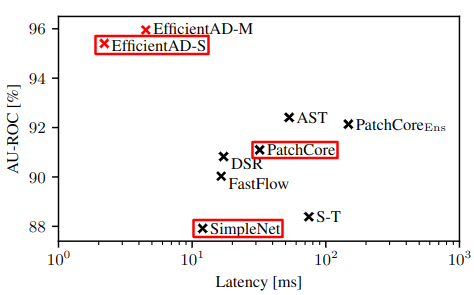
\includegraphics[width=0.4\textwidth]{bilder/overviewspeedauroc.png}
    \caption{Übersicht über AUROC und Laufzeit verschiedener Methoden ausgeführt auf Nvidia RTX A6000 GPU. \cite{efficientad}}
    \label{fig:efficientadoverview}
\end{figure}
Mit bis zu \num{99,8}\% Instanzklassifiziergungsgenauigkeit auf dem Datensatz MvTecAD ist es die Methode mit der höchsten\
Genauigkeit auf diesem Datensatz. \cite{paperswithcode}\\
Es kombiniert dabei verschiedene Methoden, die in anderen Veröffentlichungen schon erfolgreich eingesetzt wurden.\
So wird ein zweiteiliger \glqq Student-Teacher\grqq{}-Ansatz verwendet.\
Zum einen erkennen wir eine modifizierte Variante der Exktraktion von Featuren durch ein auf ImageNet implizit vortrainiertem Netz\
(Wissens-Distillation). Der andere Teil setzt auf einen Student-Teacher-Ansatz auf Basis eines Autoencoder, der die Aufgabe hat, nominale Merkmale\
zu rekonstruieren. Beide Konzepte werden in diesem Kapitel noch genauer erläutert.\\
Die Implementierung erfolgt dabei beinahe ausschließlich mithilfe von CNNs. Nur die finale Bestimmung des Anomalie-Scores und der Anomaliekarte,\
die, wie gezeigt werden wird, kaum laufzeitkritisch ist, wird ohne die Verwendung von CNNs realisiert.\
Da moderne GPUs äußerst schnelle Inferenz von CNNs ermöglichen, gehört diese Methode zu den am schnellsten ausführbaren Methoden im Bereich\
der Unüberwachten Anomaliedetekion.\cite{efficientad}\cite{paperswithcode} \\
Wie bereits gesehen werden konnte, lassen sich solche Aussagen über die Laufzeit nicht einfach übertragen, liegt keine GPU vor, wie in\
dieser Arbeit.\\
\section{Grundlage - Uninformed Students}\label{sec:GrundlageUninformedStudents}
\textcolor{green}{\textit{Abgeschlossen: 02.11. v1}}\\
Die Veröffentlichung \glqq Uninformed Students: Student-Teacher Anomaly Detection with Discriminative Latent Embeddings\grqq{}, welche am 18. März 2020\
vorgestellt wurde, präsentiert ein zentrales Konzept, welches auch in EfficientAD verwendet wird.\
Die ebenfalls von MVTec GmbH entwickelte Methode setzt somit auch auf eine Student-Teacher-Architektur.\
\subsection{Funktionsweise}
In diesem Bereich wird genauer auf die Funktionsweise von \glqq Uninformed Students\grqq{} eingegangen.\
Analog zu den bisher beschriebenen Methoden, wird zunächst der aus nominalen Bilder bestehende Trainingsdatensatz als
$\mathcal{X}_{train}={x_1, x_2, ..., x_n}$ ($\forall x \in \mathcal{X}_{train}: y_{x}=0$) definiert.\
Das Ziel ist es, ein Ensemble an \glqq Studenten\grqq{} $S_{i}$ zu erzuegen, die später in der Lage sind, Anomalien \
eines anomalen Testbildes $x_{i}\in\mathcal{X}_{test}$ und $y_{x} = 1$ mit $\forall x \in \mathcal{X}_{test}: y_{x}=\{0,1\}$ zu erkennen.\
Um eine solche Aussage zu treffen, wird die Abweichung für ein Testbild $x_{i}$ von der Ausgabe der Studenten $S_{i}$\
und der des \glqq Lehrers\grqq{} (Teacher) $T$ bestimmt. Große Abweichungen deuten dabei auf eine Anomalie hin.\
Der Teacher $T$ ist dabei ein CNN, welches auf einem großen Datensatz, wie ImageNet, vortrainiert wurde.\
Es kommen dabei keine ResNets diekt zum Einsatz, sondern einfache CNNs, die von den Autoren selbst entwickelt wurden.\
Die Architektur von Teacher $T$ und Studenten $S_{i}$ ist dabei identisch.\
\subsubsection*{Lernen von lokalen Patch Deskriptoren}
In diesem Abschnitt wird sich damit beschäftigt, wie ein Teacher $T$ in die Lage versetzt wird,
deskriptive und lokal aufgelöste Merkmale zu extrahieren. %Die Techniken, die dazu verwendet werden sind \
%\textbf{Wissens-Distillation} und \textbf{Metric-Learning}.\
$\hat{T}$ kann für beliebige $p\in\mathbb{N}$ aus einem Bild oder Bildausschnitt $\mathbf{p}\in\mathbb{R}^{p\times p\times C}$ einen eindimensionalen Feature Vektor\
erzeugen.\ 
Drei verschiedene Wege des Lernens des Teachers werden im Folgenden beschrieben.\
\paragraph*{Wissens-Distillation}\label{par:wissensdistillation}
Wie bereits ausführlich in \ref{subsec:ResNetsAsFeatureExtractor} und in den vorangegangenen Methoden beschrieben,\
dienen CNNs, die auf großen Datensätzen vortrainiert wurden, als Feature-Extraktoren für aussagekräftige und kompakte Merkmalsextraktoren.\
Um ein leichtgewichteren Featre Extraktor zu erhalten, wird das CNN $\hat{T}$ trainiert um das Verhalten eines großen, auf ImageNet vortrainierten\
CNNs $\phi$ zu imitieren. Es werden dazu Bilder aus ImageNet auf die Größe $p\times p$ ausgeschnitten und dienen als Eingangsgröße.\
Das Label könnte nun direkt aus einem Einbettungsprozess wie bei \ref{subsec:ErzeugenDerPatchFeatures} erzeugt werden, es ergeben sich\
aber Probleme durch unterschiedliche Größen der jeweiligen Ausgaben. Deshalb wird zusätzliche ein einfaches vollvernetztes neuronales Netz (MLP)\
eingesetzt, dass die Ausgaben des Netzwerkes $\phi$ auf die gewünschte Größe $d$ abbildet.\
Folgende Verlustfunktion wird verwendet, um das Netzwerk $T$ zu trainieren:\
$$
\mathcal{L}_{KD} = \left\lVert D(\hat{T}(\mathbf{p}))-\phi(\mathbf{p}) \right\rVert_{2}^{2}
$$
$\hat{T}$ ist jedoch auf eine Eingabe von $p\times p$ Pixeln beschränkt, soll ein eindimensionaler Feature Vektor erzeugt werden. \
Das Netzwerk $\hat{T}$ muss dementsprechend noch in die Lage versetzt werden, mit größeren Bildern umzugehen. Die Autoren dieser Veröffentlichung \
gehen dabei nach \cite{bailer2018fast} vor und erhalten so einen effizienten Feature Extraktor $T$.\
Für $\hat{T}$ werden drei verschiedene Architekturen verwendet, die sich in ihrer Komplexität und der Größe des rezeptiven Feldes ($p\in\{17,33,65\}$) unterscheiden. \
Für weitere Details wird an dieser Stelle auf die Veröffentlichung \cite{bailer2018fast} verwiesen, weil es hier vor allem um das Konzept \
und dessen Erläuterung gehen soll.\\
Das für die Wissens-Distillation verwendete Netzwerk $\phi$ ist ein ResNet-18, welches auf ImageNet vortrainiert wurde. Es wird dabei der 1D-Feature-Vektor \
aus der letzten Schicht des ResNets (\glqq flatten\grqq{} in \ref{fig:ResNetPyramid}) verwendet. Dieser 512 Einträge fassender 1D-Vektor wird mithilfe von $D$ auf $d=128$\
Einträge komprimiert. Es sei angemerkt, dass es sich hierbei um die Werte aus der Originalveröffentlichung handelt und andere Wertekombinationen ebenfalls möglich sind. \
\paragraph*{Metrisches Lernen}\label{par:metrischeslernen}
Beim metrischen Lernen wird zunächst ein Triplet aus Patches $(\mathbf{p}, \mathbf{p}^{+}, \mathbf{p}^{-})$ erzeugt. Das Ausgangspatch $\mathbf{p}$\
wird dabei durch einen zufällig ausgeschnittenen Bildausschnitt aus einem Bild aus dem Trainingsdatensatz erzeugt.\
$\mathbf{p}^{+}$ ist eine mit Gauß'schen Rauschen und veränderte Helligkeit augmentierte Version von $\mathbf{p}$.\
Bei $\mathbf{p}^{-}$ handelt es sich um einen Bildausschnitt aus einem anderen Bild aus dem Trainingsdatensatz.\
Die Verlustfunktion für das metrische Lernen ist dann gegeben durch: \
$$
\mathcal{L}_{M} = \max\left\{0,  \delta + \delta^{+}-\delta^{-}\right\}
$$
$$
\delta^{+}=\left\lVert \hat{T}(\mathbf{p})-\hat{T}(\mathbf{p}^{+}) \right\rVert_{2}^{2}
$$
$$
\delta^{-}=\min\left\{\left\lVert \hat{T}(\mathbf{p})-\hat{T}(\mathbf{p}^{-}) \right\rVert_{2}^{2}, \left\lVert \hat{T}(\mathbf{p}^{+})-\hat{T}(\mathbf{p}^{-}) \right\rVert_{2}^{2} \right\}
$$
Dabei bezeichnet $\delta>0$ einen Randparameter, der einen Hyperparameter bzgl. des Trainings darstellt. \
Minimiert man diese Verlustfunktion, so wird das Netzwerk $\hat{T}$ in die Lage versetzt, ähnliche Patches in einem Feature Raum nahe beieinander zu platzieren und die distinkten\
Patches weiter voneinander zu entfernen. Es wird also die diskriminative Fähigkeit des Netzwerkes $\hat{T}$ gestärkt.\
\paragraph*{Kompaktheit der Merkmale}\label{par:kompaktheitdermerkmale}
Um eine kompakte und möglichst wenige redundante Representation der Merkmale zu erhalten, wird ein weitere Verlustfunktion eingeführt. \
$$
\mathcal{L}_{C}\left(\hat{T}\right) = \sum_{i\neq j} c_{ij} 
$$
Die skalaren Parameter $c_{ij}$ bezeichnen dabei die Einträge der Korrelationsmatrix über alle $\hat{T}\left(\mathbf{p}\right)$ für sämtliche $\mathbf{p}$ im aktuellen Mini-Batch des \
Trainings. Indem die Einträge auf der Diagonalen nicht minimiert werden, die Einträge außerhalb der Diagonalen jedoch schon, wird eine Darstellung gefördert, \
die die einzelnen Merkmale, welche $d$-fach im Feature Vektor gebündelt sind, entkoppelt, also unabhängig voneinander macht. \\
Die finale Verlustfunktion ergibt sich dann aus einer Linearkombination dieser drei Verlustfunktionen: \
$$
\mathcal{L}_{T} = \lambda_{KD}\mathcal{L}_{KD} + \lambda_{M}\mathcal{L}_{M} + \lambda_{C}\mathcal{L}_{C}, \quad \lambda_{KD}, \lambda_{M}, \lambda_{C} \in \mathbb{R}^{+}
$$
Die Faktoren $\lambda_{KD}, \lambda_{M}, \lambda_{C}$ sind dabei Hyperparameter, die das Training beeinflussen. \
\subsubsection*{Lernen der Studenten}
Nun wird sich mit dem Training der Studenten $S_{i}$ beschäftigt. Diese sollen in die Lage versetzt werden, \
nominale Patches in der selben Weise, wie der Teacher $T$ zu extrahieren, also dessen Ausgabe auf nominalen Bildern zu imitieren.\
Liegt ein anomales Bild vor, so soll die Ausgabe der Studenten möglichst stark von der des Teachers abweichen.\\
Zunächst wird die Ausgabe des trainierten Teachers $T$ über alle Bilder in $\mathcal{X}_{train}$ erzeugt. Aus den so entstandenen Merkmalsvektoren wird dann\
der Mittelwert $\boldsymbol{\mu}\in\mathbb{R}^{d}$ und die Standardabweichung $\mathbf{\sigma}\in\mathbb{R}^{d}$ komponentenweise bestimmt.\
Für jede mögliche Position $(h,w)$ mit $h\in\{1,...,h^{*}\}$ und $w\in\{1,...,w^{*}\}$ wird dann die Ausgabe $y$ der Studenten $S_{i}$ bestimmt\
und als Gaußverteilung $P\left(\mathbf{y}|\mathbf{p}_{h,w}\right)=\mathcal{N}\left(\mathbf{y}|\boldsymbol{\mu}^{S_{i}}_{h,w},s\right)$ mit konstanter\ 
Kovarianz $s\in\mathbb{R}$ modeliert. $\boldsymbol{\mu}^{S_{i}}_{h,w}$ ist hierbei die Prädiktion von $S_{i}$ zur Stelle $\left(h,w\right)$.\
Sei nun $\mathbf{y}^{T}_{h,w}$ die von den Studenten zu prädizierende Zielgröße, also die Ausgabe des trainierten Teachers, ergibt sich damit folgende\
Verlustfunktion für das Training des Studenten:\\
$$
\mathcal{L}\left(S_{i}\right)= \frac{1}{h^{*}w^{*}} \sum_{\left(h,w\right)\in \left\{1,...,h^{*}\right\} \times \left\{1,...,w^{*}\right\}} \left\lVert \boldsymbol{\mu}^{S_{i}}_{h,w} - \left(\mathbf{y}_{h,w}^{T}-\boldsymbol{\mu}\right)diag\left(\boldsymbol{\sigma}^{-1}\right) \right\rVert_{2}^{2}
$$
$diag\left(\boldsymbol{\sigma}\right)^{-1}$ ist dabei die Inverse der Diagonalen der Matrix, die mit den Werten aus $\boldsymbol{\sigma}$ gefüllt ist.\
\subsubsection*{Bestimmen des Anomaliegrades}\label{subsubsec:bestimmendesanomaliegradesUninformedStudents}
Nach dem Training der Studenten bis zur Konvergenz, wird für jeden Position $(h,w)$ eines Bildes eine Gauß-Mixtur bestimmt. Dies geschieht über alle Studenten des Ensembles, die alle gleichgewichtet eingehen. \
Damit kann auf zwei verschiedene Wege ein Anomaliegrad bestimmt werden. \\
Zunächst lässt sich der Regressionsfehler zwischen der Ausgabe des Teachers und dem Mittelwert der Ausgaben der Studenten bestimmen. \
$$
e_{h,w} = \left\lVert \boldsymbol{\mu}_{h,w} - \left(\mathbf{y}_{h,w}^{T}-\boldsymbol{\mu}\right)diag\left(\boldsymbol{\sigma}^{-1}\right) \right\rVert_{2}^{2} 
$$
$\boldsymbol{\mu}_{h,w}$ ist hierbei der Mittelwert der Ausgaben der Studenten an der Position $(h,w)$ ($\boldsymbol{\mu}_{h,w}=\frac{1}{M} \sum_{i=1}^M\boldsymbol{\mu}_{h,w}^{S_i}$). \
Die Idee ist nun, dass ein hoher Regressionsfehler auf eine Anomalie hinweist, weil die Studenten nicht in der Lage sind, \
die Ausgabe des Teachers zu imitieren. \\
Eine andere Möglichkeit der Bestimmung eines Anomaliegrades ist es, die Unsicherheit der Prädiktionen der Studenten zu betrachten.\
Dies basiert auf der Annahme, dass die Augaben der Studenten auf nominalen Bildern eine geringere Varianz aufweisen, als auf anomalen Bildern, weil\
diese Ungesehenes beinhalten, für das das jeder Student $S_{i}$ eine andere, zufällig streuende Prädiktion ausgibt.\
Quantitativ kann das wie folgt formuliert werden:\
$$
v_{h,w}=\frac{1}{M} \sum_{i=1}^M\left\|\boldsymbol{\mu}_{h,w}^{S_i}\right\|_2^2-\left\|\boldsymbol{\mu}_{h,w}\right\|_2^2
$$
Mit einer Normalisierung der jeweiligen Größen $e_{h,w}$ und $v_{h,w}$ mithilfe der Mittelwerte und Standardabweichung über alle Positionen $(h,w)$ folgt \
schließlich das für ein Studeten-Teacher-Paar finale Anomaliemaß für die Position $(h,w)$: \
$$
\tilde{s}_{h,w}=\tilde{e}_{h,w}+\tilde{v}_{h,w}=\frac{e_{h,w}-e_\mu}{e_\sigma}+\frac{v_{h,w}-v_\mu}{v_\sigma} .
$$
Weitergehend kann nur ein Ensemble an Student-Teacher-Paaren verwendet werden, um die Anomalieklassifikation zu verbessern. \
Sinnvoll ist es, solche Paare zu trainieren, die unterschiedliche rezeptive Felder $p$ aufweisen. Dann können Anoamlien unterschiedlicher Größe \
detektiert werden, ohne dass ein Hoch oder Runterskalieren des Bildes notwendig ist, was immer mit einem Informationsverlust einhergeht. \
Für $L$ Student-Teacher-Paare ergibt und die die jeweiligen Anomliegrade $\tilde{s}_{h,w}^{(l)}$, ergibt sich dann \
$$
s_{h,w}=\frac{1}{L}\sum_{l=1}^L\tilde{s}_{h,w}^{(l)} .
$$
\subsection{Ergebnisse und Diskussion}
Es handelt sich bei dieser Methode um die älteste in dieser Arbeit beschriebene Methode.\
Viele Erkentnisse, die in den darauffolgenden Jahren durch zahlreiche Veröffentlichungen gewonnen wurden, fehlten\
den Autoren dieser Veröffentlichung. So wurde als Lernziel für den Teacher $T$ und die Wissensdistillation ein ResNet 18 verwendet, dessen Feature dann mittels PCA in die richtige Dimension gebracht wurde.\
Heute ist bekannt, dass tiefere Netze bessere Feature Extraktoren sind und PCA keine geeignete Methode ist, um Patch Feature zu reduzieren. Letzteres wurde z.B. in PaDiM festgestellt, aber auch in qualitativen Untersuchungen in dieser Arbeit.\
Auch das metrische Lernen erweist sich als nicht hilfreich, wie bereits die Autoren selbst in ihrer Veröffentlichung feststellen.\\
Vor diesem Hintergrund ist die erzielte Genauigkeit dennoch beachtlich und entspricht in etwa den Ergebnissen von SPADE. Der Fokus in dieser Arbeit lag nicht auf einer\
Instanzklassifiziergung, sondern auf der Segmentierung, weswegen hierfür weder eine Methode, noch Ergebnisse veröffentlicht wurden. Aufgrund der pixelweisen Metriken, die in der Veröffentlichung angeben sind und an dieser Stelle\
nicht weiter besprochen werden, lässt sich diese Aussage treffen.\\
Auch Aussagen zur Laufzeit müssen qualitativ erfolgen. Es ist nicht davon auszugehen, dass durch die Vielzahl an Elementen ($M=3$ und $L=3$) die Laufzeit geringer ist, als bei den anderen Methoden.\
Insgesamt müssten bei einem solchen Konfiguration, wie sie in der Veröffentlichung angegeben ist, 9 CNNs auf einem Bild ausgeführt werden.\\
Viel wichtiger als die tatsächlichen Ergebnisse, sind aber die Impulse, die durch diese Arbeit gesetzt wurden. Folgende Erkentnisse sind hierbei besonders hervorzuheben:\
\begin{itemize}
    \item Eine Feature Exktrattion durch Wissensdistillation ist möglich und ermöglicht spezifisch angepasste Feature Extraktoren, die auf die Aufgabe zugeschnitten sind.\
    \item Ein Student-Teacher Ansatz ist eine geeignete Methode, um Anomalien zu detektieren.\
    \item Verschieden aufgelöste Feature Maps können zu einer Verbesserung der Anomaliedetektion führen.\
\end{itemize}
In nachfolgendem Abschnitt zur Funktionsweise von EfficientAD werden einige dieser Erkentnisse aufgegriffen und weiterentwickelt.\
\section{Funktionsweise von EfficientAD}\label{sec:funktionsweisevonEfficientAD}
\textcolor{green}{\textit{Abgeschlossen: 02.11. v1}}\\
In diesem Abschnitt wird die Funktionsweise der Methode EfficientAD beschrieben. Es wird hauptsächlich das Konzept des \
Student-Teacher Designs, das in \ref{sec:GrundlageUninformedStudents} beschrieben wurde, verwendet. \
Dabei gibt es zwei, konzeptionell unterschiedliche Student-Teacher Paare, die jeweils unterschiedliche Aufgaben erfüllen. \
\subsection{Feature Extraktion}\label{subsubsec:featureextraktionEfficientad}
Ein wesentlicher Unterschied zu PatchCore und SimpleNet ist, dass für die Feature Exktration \
nicht auf explizit auf ein vortrainiertes ResNet gesetzt wird. \ 
Zwar wird diese Grundidee immer noch beibehalten, insofern, als dass ein solches ResNet verwendet wird, \
um den eigentlichen Feature Extraktor zu trainieren. Während der Inferenz wird jedoch kein ResNet verwendet. \
Stattdessen kommt ein sogenannter \textbf{Patch Description Network (PDN)} zum Einsatz, welches mithilfe von Wissens-Distillation \ 
trainiert wird. Es besteht aus lediglich vier Convolutional-Layern, die in \ref{fig:pdn} dargestellt sind.\\
\begin{figure}[h]
    \centering
    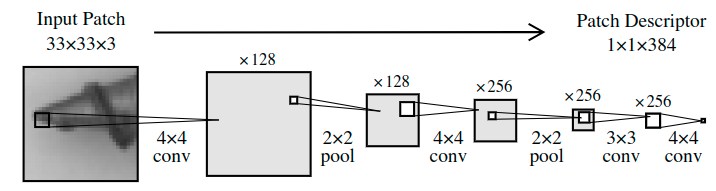
\includegraphics[width=0.8\textwidth]{bilder/pdn.png}
    \caption{Skizze der Architektur des Patch Description Networks (PDN). \cite{efficientad}}
    \label{fig:pdn}
\end{figure}
In \ref{fig:pdn} zu sehen, ist, dass die Ausgabe eines PDN 384-dimensionale Feature-Vektoren sind, deren rezeptives Feld exakt $p=33$ Pixel beträgt.\
Dies entspricht der Idee, die bereits drei Jahre zuvor in \glqq Uninformed Students\grqq{} \cite{uninformedstudents} vorgestellt wurde.\
Im Falle eines ResNets als Feature Exktraktor kann das rezeptive Feld selten grenzscharf bestimmt werden, wodurch sich das PDN für Segmentierungsaufgaben\
in dieser Hinsicht besser eignet. \\
Eine räumliche Dimensionsreduktion findet durch ein schrittweises Average-Pooling nach den ersten beiden Convolutional-Layers statt. Die geringere Dimension der\
Feature Maps sorgen für eine schnellere Laufzeit. Wie noch zu sehen sein wird, ist diese Dimensionsreduktion allerdings deutlich zurückhaltender, als zum Beispiel bei ResNet-Architekturen.\\
Durch den vollständig aus Convolutional- und Pooling-Layern bestehende Aufbau des PDN, ist es möglich, alle Feature Vektoren eines Bildes in einem\
Durchlauf zu extrahieren.\
Es stehen zwei verschiende PDNs zur Verfügung, welche sich in ihrere Größe und daraus resultierend, ihrer Laufzeit unterscheiden.\
Insbesondere die Anzahl an Filter in den Convolutional-Layern unterscheidet sich, also die Anzahl an Channels. Diese ist im Falle des größeren Netzes \
deutlich höher. Für Details hierzu wird auf die Veröffentlichung \cite{efficientad} und Tabelle 5 bzw. 6 verwiesen.\\
Wie bereits erwähnt, erfolgt das Training des PDNs mithilfe von Wissens-Distillation von einem vortrainierten ResNet.\
In \ref{par:wissensdistillation} wurde bereits beschrieben, wie ein solcher Distillationsprozess aussieht.\
Definieren wir den PDN als $T:\mathbb{R}^{3\times 256\times 256}\rightarrow \mathbb{R}^{384\times 64\times 64}$ benötigen wir einen vortrainierten \
Feature Extraktor $\phi:\mathbb{R}^{3\times W\times H}\rightarrow \mathbb{R}^{384 \times 64\times 64}$, der auf ImageNet vortrainiert wurde. \
Die Kantenlängen $W$ und $H$ sind dabei so zu wählen, dass die Ausgabe des Feature Extraktors $\phi$ $64\times 64$ Pixel groß ist.\
Hierzu eignet sich ein Feature Extraktor, wie in \ref{subsec:ErzeugenDerPatchFeatures} bei der Methode PatchCore verwendet, ideal.\
Es wird auch in der Veröffentlichung der Einbettungsprozess aus \ref{subsec:ErzeugenDerPatchFeatures} verwendet und ein Wide ResNet 101 \cite{wideresnet}.\
Die Verlustfunktion für das Training des PDNs auf mit einem Bild $x\in\mathcal{X}_{train}$ ergibt sich dann einfach zu:\
$$
\mathcal{L}= \left\lVert T(x)-\phi(x) \right\rVert_{2}^{2}
$$
$\mathcal{X}_{train}$ ist hierbei aus dem ImageNet Datensatz entnommen. Es handelt sich also um einen $L2$-Loss. \ 
Die Auflösung $H \times W$ der Bilder aus ImageNet beträgt in diesem Fall, also mit einem Wide ResNet 101, $512\times 512$ Pixel. \\
\subsection{Reduzierter Student-Teacher Ansatz}
Die in \ref{sec:GrundlageUninformedStudents} beschriebene Methode \glqq Uninformed Students\grqq{} wird in EfficientAD in einer reduzierten Form verwendet.\
Es wird kein Ensemble an Studenten verwendet, sondern nur ein einzelner Student, was $M=1$ in \ref{subsubsec:bestimmendesanomaliegradesUninformedStudents} entspricht.\
Ebenfalls kommt lediglich eine Student-Teacher Paarung in diesem Schritt zum Einsatz. Gegenüber der Veröffentlichung \glqq Uninformed Students\grqq{}\cite{uninformedstudents}\ 
ist das eine weitere Vereinfachung. Diese dienen in erster Linie einer kürzeren Laufzeit.\\
Der Teacher $T$ ist dabei durch das PDN, trainiert durch Wissensdistillation, gegeben. Für den Studenten $S$ wird die Architektur identisch übernommen.\\
Es wird somit auch auf eine asymetrische Architektur verzichtet, wie sie erfolgreich in \cite{ast} angewandt wurde.\
Stattdessen wird auf eine angepasste Verlustfunktion zurrückgegriffen, die im Folgenden beschrieben wird.\\
Grundsätzlich besteht die Schwierigkeit beim Trainieren eines Student-Teacher Paares darin, den Studenten zwar soweit zu trainieren, dass er in der Lage ist,\
das Verhalten des Teachers auf nominalen Beispielen möglichst genau zu imitieren, aber dennoch nicht genug generalisiert zu haben, dies auch in einem anomalen Fall zu tun.\
Es entsteht ein Trade-Off, der in dieser Veröffentlichung clever gelöst wird.\\
So wird zunächst ein Verfahren eingeführt, dass nur Bereiche im Bild für das Anpassen der Parameter mithilfe von Backpropagation verwendet, welche \
besonders große Abweichungen zwischen der Ausgabe des Teachers und des Studenten aufweisen. Geringfügige Abweichungen werden ignoriert.\\
Formal wird dazu ein Trainingsbild $x \in \mathcal{X}_{train}$ verwendet, um die Ausgabe sowohl des Studenten $S(x)$, als auch des Teachers $T(x)$ zu bestimmen.\
Dabei ist $T(x), S(x) \in \mathbb{R}^{C \times H \times W}$. Daraus wird dann die quadratische Differenz $D_{c,w,h} = \left(T(x)_{c,w,h}-(S(x)_{c,w,h})\right)^{2}$\
für jedes Element $(c,h,w)$ bestimmt. Der Idee folgend, nur die größten Differenzen eingehen zu lassen, wird anschließend ein Schwellwert $d_{hart}$ berechnet,\
der von einem Hyperparameter $p_{hart} \in \left[0,1\right]$ abhängt. Dieser bestimmt, wie groß die Menge an Elementen aus $D_{c,w,h}$ ist, die für das Training verwendet werden.\
Es gilt, dass $d_{hart}$-Quantil $d_{hart}$ ist. Für $p_{hart}=\num{0,999}$ werden laut \cite{efficientad} etwa 10\% der Elemente aus $D_{c,w,h}$ für das Training verwendet.\
Würde $p_{hart}=0$ gewählt, so würden alle Elemente $D_{c,w,h}$ für das Training verwendet. \ Konkret wird dann die Verlustfunktion $\mathcal{L}_{hart}$ zum Durchschnitt\
über alle Werte aus $D$ bestimmt, für die gilt, dass $D_{c,w,h} \geq d_{hart}$.\\
In der Praxis führt dieser Ansatz dazu, dass nur wesentliche Bereiche im Bild für das Training verwendet werden. Veranschaulicht ist das in nachfolgender Abbildung, welche der\
Veröffentlichung entnommen wurde (\ref{fig:hardthreshold}). Es ist zu erkennen, dass Objektbereiche in $\mathcal{L}_{hart}$ eingehen, der Hintergrund hingegen bereits vom Studenten\
gut imitiert wird und somit nicht mehr in die Verlustfunktion eingeht.\\
\begin{figure}[h]
    \centering
    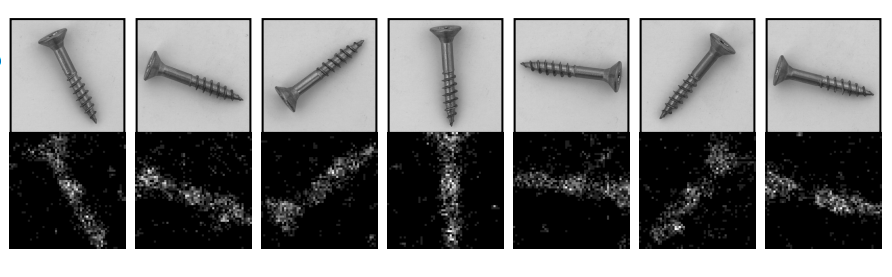
\includegraphics[width=0.8\textwidth]{bilder/hardloss.png}
    \caption{Veranschaulichung der \glqq Hard Loss\grqq{}-Filterung für $\mathcal{L}_{hart}$. Obere Reihe stellt Trainingsbilder dar, Untere die Masken. Alle dunklen Bereiche werden ignoriert, helle Bereiche werden zum Training verwendet. \cite{efficientad}}
    \label{fig:hardthreshold}
\end{figure}
Zusätzlich zu dieser speziellen Verlustfunktion, die für das Training des Studenten verwendet wird, wird ein Strafterm eingeführt, der den Studenten daran hindert,\
den Teacher auf Bildern, die nicht Teil der nominalen Trainingsdaten sind, zu imitieren.\ 
In einem klassischen Setup würde der Student vom Teacher nur mit Bildern lernen, die nominal und aus der Zieldomäne stammend sind. Der Teacher hingegen würde auf einem größeren,\ 
breter gefassten Datensatz trainiert werden, zum Beispiel mit ImageNet.\ 
In dieser Veröffentlichung wird der Student zusätzlich auf Bildern trainiert, die aus dem ImageNet Datensatz stammen.\
Konkret wird in jedem Trainingsschritt ein Bild $x_{imagenet}$ aus ImageNet zufällig ausgewählt und mit der Verlustfunktion $\mathcal{L}_{Strafterm}=\frac{\sum_{c}\lVert S(x_{imagenet})_{c} \rVert^{2}_{F}}{HWC}$\ 
ein Strafterm bestimmt. Es wird hierfür die Frobenius-Norm über alle Kanäle verwendet. Dieser Strafterm verhindert, dass der Student auf Bildern, die nicht aus der Zieldomäne stammen,\
generalisiert.\\
Die finale Verlustfunktion für den Studenten ergibt sich dann zu:\
$$
\mathcal{L}_{Student}= \mathcal{L}_{hart} + \mathcal{L}_{Strafterm} %TODO --> besseren Namen für "hart"
$$
Eine detailierte Aufschlüsslung des gesamten Trainingsprozesses ist in \cite{efficientad} im Appendix A.1 und Algorithus 1 zu finden.\\
\subsection{Erkennen logischer Anomalien}\label{subsec:erkennenlogischeranomalien}
Wie bereits in der Einleitung zu diesem Kapitel erwähnt, ist EfficientAD in der Lage, neben strukturellen Anomalien, auch logische Anomalien zu erkennen.\
Weil bei PatchCore und SimpleNet keine globale Strukturinformationen verwendet werden, sondern immer nur bereichsweise analysiert wird, ist es nur sehr eingeschränkt möglich\
mit diesen Methoden logische Anomalien zu erkennen. In \ref{sec:DatensatzMVTecAD} wurde bereits erwähnt, dass der MVTec AD Datensatz im Wesentlichen keine logischen Anomalien enthält\
und die Zielsetzung dieser Arbeit nicht die Erkennung logischer Anomalien ist. Deshalb wird diese interessante Fähigkeit von EfficientAD hier nicht weiter betrachtet.\
Auf dem Datensatz MVTec LOCO AD, der ebenfalls in \ref{sec:DatensatzMVTecAD} Erwähnung findet und hautpsächlich logische Anomalien enthält, ist die Methode EfficientAD\
die beste bislang veröffentlichte Methode (Stand Oktober 2023). \cite{mvtecadloco} \\
Um solche Anomalien zu erkennen, wird ein Autoencoder verwendet, um die logischen Zusammenhänge nominaler Bilder zu erlernen. Es wird sich dabei vor allem an der Methode \glqq GCAD\grqq{} \
orientiert \cite{gcad}, die sich mit dem Erkennen logischer Anomalien mithilfe von Autoencodern beschäftigt. Weil dies nicht Schwerpunkt dieser Arbeit ist, wird auf eine Erläuterung \
der Methode GCAD hier verzichtet. Die wesentlichen Aspekte von GCAD finden sich ohnehin in dem hier Beschriebenen wieder.\\
Ebenfalls wird ein Student-Teacher Paar gebildet. Auch hier wird der Student $A$, der durch den Autoencoder implementiert wird, trainiert, um die Ausgabe des Teachers $T$ zu imitieren. \
Formal ergibt sich die Verlustfunktion für das Training des Autoencoders für ein Bild $x$ zu: \
$$
\mathcal{L}_{AE} = \frac{\sum_{c}\left\lVert A(x)_{c}-T(x)_{c} \right\rVert_{F}^{2}}{HWC}
$$
Auch hier ist $T(x), A(x) \in \mathbb{R}^{C \times H \times W}$ und die Frobenius-Norm wird über alle Kanäle verwendet. Das Bild $x$ ist dabei ein Bild aus dem Trainingsdatensatz, der in \
diesem Fall ausschließlich aus nominalen Bildern der Zieldomäne besteht.\\
Im Gegensatz zu den PDNs, die immer nur ein endlich großes rezeptives Feld haben, welches im Falle der PDNs sogar exakt definiert ist, wird vom Autoencoder das gesamte Bild betrachtet.\
Es muss möglichst viel der Bildinformation durch ein \glqq Bottleneck\grqq{} (dt.: Flaschenhals) bringen, um eine Rekonstruktion des Bildes zu ermöglichen. Dieses Bottleneck ist\
dabei lediglich 64 Kanäle fassend, wodurch eine Komprimierung erzwungen wird.\\
Man spricht Im Zuammenhang mit Autoencodern vom Encoder, der die Bildinformation auf einen niedrigdimensionalen Vektor, das Bottleneck, abbildet und dem Decoder, der diesen Vektor wieder\
auf eine größere Dimension abbildet. Diese Zieldimension entspricht dabei nicht der Auflösung des Eingangsbildes, sondern der Auflösung der Patch Feature Vektoren.\\
Auf Bildern mit logischen Anomalien ist die grundsätzliche Struktur des Bildes verschieden zur nominalen Struktur. Da der Autoencoder jedoch aus dem Training nur\
nominale Bilder zu sehen bekommt und diese grundsätzliche Struktur implizit zur möglichst fehlerfreien Rekonstruktion erlernt und ausgenutzt hat, wird der\
Autoencoder nicht in der Lage sein, eine Abweichung der nominalen Struktur ebenfalls korrekt zu rekonstruieren.\\
Autoencoder haben im Allgemeinen die Schwäche, dass die Rekonstruktionen von fein aufgelösten Bilddetails nicht gut gelingt. Dies ist auch hier der Fall.\
Um falsche Positive, also scheinbare Anomalien, die durch eine schlechte Rekonstruktion solcher feiner Strukturen entstehen würden, zu vermeiden, wird die Anzahl der\
Ausgangskanäle des Studenten $S$ verdoppelt und trainiert, die Ausgabe des Autoencoders zu imitieren.\
Definiert man nun den Teil des Studenten, der mit dem Autoencoder korrespondert mit $S^{\prime}$ und $S^{\prime}(x) \in \mathbb{R}^{C \times H \times W}$ als die Ausgabe\
dieses Teils des Studenten, ergibt sich die Verlustfunktion für das Training des Studenten $S^{\prime}$ zu:\
$$
\mathcal{L}_{AE} = \frac{\sum_{c}\left\lVert S^{\prime}(x)_{c}-A(x)_{c} \right\rVert_{F}^{2}}{HWC}
$$
Somit lernt der Student $S^{\prime}$, die systematischen Rekonstruktionsfehler des Autoencoders $A$ mit, wodruch diese nicht mehr zu falschen Positiven führen.\
Außerdem ist der Student $S^{\prime}$ Teil des PDNs, welches ein rezeptives Feld von $p=33$ Pixeln hat. Es ist also nicht in der Lage größere Strukturen zu erkennen und\
somit in aller Regel nicht beeinfluss von logischen Anoamlien.\\
\subsection{Bestimmen des Anomaliegrades}\label{subsec:efficientadbestimmenanomaliegrades}
In beiden oben genannten Paaren, also Autoencoder $A$ und Student $S^{\prime}$ sowie PDN $T$ und Student $S$, kann die Differenz der Ausgaben als Anomaliemaß verwendet werden.\
Konkret wird die pixelweise quadratische Differenz der Ausgaben berechnet.\
Es entstehen somit zwei Anomaliekarten, die im Folgenden als lokale Anomliekarte für die Differenz von $S$ und $T$ und als globale Anomaliekarte für die Differenz von $S^{\prime}$ und $A$ bezeichnet werden. \
In folgender, der Veröffentlichung entnommenen, Abbildung ist das unterschiedliche Verhalten dieser beiden Anomaliekarten veranschaulicht.\\
\begin{figure}[h]
    \centering
    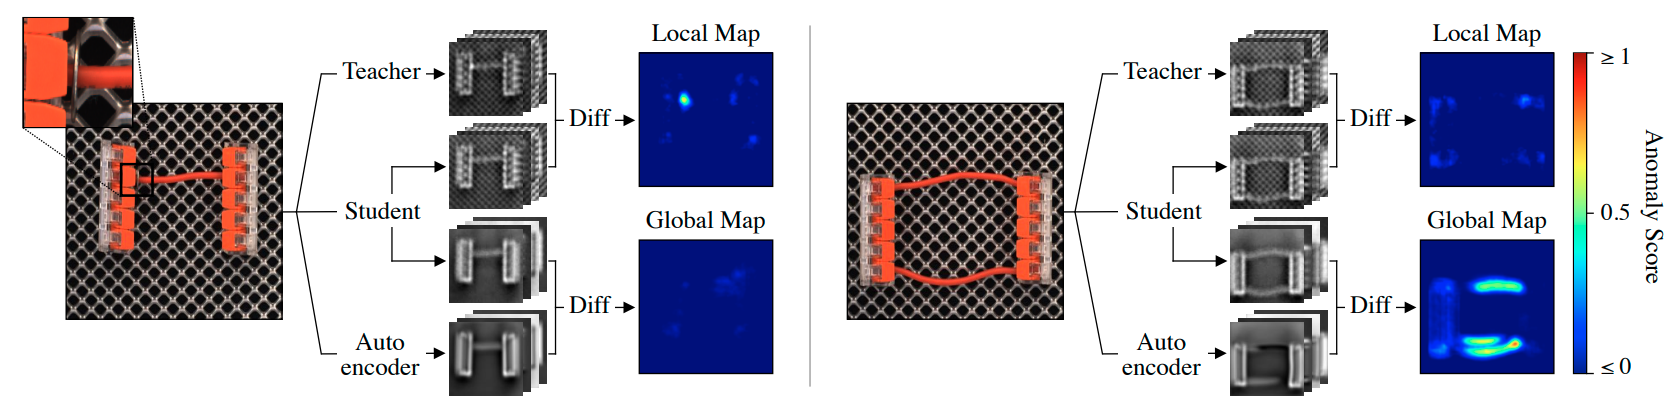
\includegraphics[width=0.8\textwidth]{bilder/localglobal.png}
    \caption{Veranschaulichung der Unterschiede zwischen lokaler und globaler Anomaliekarte. \cite{efficientad}}
    \label{fig:localglobal}
\end{figure}
Es handelt sich hierbei um zwei Beispielbilder aus dem bereits erwähnten Datensatz MVTec LOCO AD. Auf der linken Seite ist ein Testbild zu sehen, welches einen kleinen, strukturellen Defekt aufweist. \
Die globale Struktur des Bildes ist aber in Ordnung. Alle Baulteile sind an Stellen, an denen man sie erwarten würde.\
Dementsprechend ist die Differenz, die unten in der \glqq Global Map\grqq{} abgebildet ist, sehr gering. Dies lässt also keinen Schluss auf eine Anomalie zu.\
Die lokale Anomaliekarte hingegen, die oben zu sehen ist, zeigt eine deutlich erhöhte Differenz an der Stelle des Defekts, was wiederum eindeutig auf die tatsächlich\
existierende, strukturelle Anomalie hinweist.\\
Auf der rechten Seite ist ein Testbild zu sehen, welches eine logische Anomalie aufweist. Die globale Anomaliekarte zeigt hier eine deutlich erhöhte Differenz,\
während die lokale Anomaliekarte keine erhöhte Differenz aufweist.\\
Nun sollen aber nicht logische und strukturelle Anomlien voneinander unterschieden werden, sonder eine resultierende, finale Anomaliekarte soll erstellt werden.\
Dies geschieht, naheliegenderweise, durch eine Kombination der beiden Anomaliekarten.\ 
Es müssen allerdings unterschiedliche Rauschniveaus der beiden Anomaliekarten berücksichtigt werden, um keine falschen Positive zu erzeugen.\
Um das Ausmaße des Rauschens für beide Karten zu bestimmen, werden ungesehene Bilder aus dem Trainingsdatensatz verwendet. Mit diesen wird eine Menge\
aller auftretenden Differenzen jeweils für beide Karten bestimmt. Mithilfe dieser Mengen werden dann die Quantile $q_{a}$ und $q_{b}$ bestimmt, die das Rauschniveau der jeweiligen Karte beschreiben. \
Abschließend wird jeweils eine lineare Transformation bestimmt, die die den Wert $q_{a}$ auf 0 und den Wert $q_{b}$ auf \num{0,1} abbildet.\
Zu den einzelnen Zahlenwerten sind Ablation Studien in \cite{efficientad} zu finden.\\
Die finale Anomliekarte ergibt sich dann einfach aus der Addition der beiden Anomaliekarten.  
\section{Ergebnisse und Diskussion der Originalmethode}\label{subsec:efficientadergebnisseunddiskussion}
\textcolor{green}{\textit{Abgeschlossen: 02.11. v1}}\\
Trotz des leichtgewichtigen Aufbaus des PDNs, ist eine Beschleunigung der Feature Extraktion gegenüber einem kleinen ResNets nicht zu erwarten.\
Dies liegt vor allem daran, dass die Feature Maps in frühen Schichten des ResNets gegenüber dem Eingangsbild stark herunterskaliert werden. Zwar wird dies auch\
bei den hier verwendeten PDNs getan, aber in einer weniger stark ausgeprägten Weise.\
Bereits nach der \glqq Layer1\grqq{} ist bei einem ResNet, wie Abb. \ref{fig:ResNetPyramid} zu entnehmen ist, die räumliche Auflösung (Anzahl an Pixeln) $16$ mal kleiner als die des Eingangsbildes.\
Beim PDN wird sie durch ein Average-Pooling mit Kernelgröße $\texttt{k}=2$, Schrittweite $\texttt{s}=2$ lediglich um den Faktor $4$ reduziert.\
Weil somit der Tensor der Feature Maps, dessen Größe bei einem CNN maßgeblich die Anzahl an Berechnungen bestimmt, damit bei einem PDN deutlich größer ist,\
ist eine Beschleunigung der Feature Extraktion kaum zu erwarten.\ 
Der Vorteil eines solchen Ansatzes ist, dass die Auflösung der finalen Anomaliekarte auch ohne ein Hochskalieren verhältnismäßig groß bleibt.\
Insbesondere für eine Segmentierungsaufgaben ist das eine wertvolle Eigenschaft, die für diese Arbeit allerdings keine explizite Rolle spielt.\\
Vergleicht man die Laufzeiten gesamter ResNets aus Tab. \ref{tab:model-runtimes} mit denen der PDNs bestätigt sich die Vermutung, dass die Laufzeit\
nicht geringer als bei einem ResNet 18 oder 34 ist. Für ein Eingangsbild der Dimension $224\times 224$ ist die Laufzeit auf der Desktop-CPU (AMD Ryzen R5 5600X, mittlere Spalte)\
mit \num{42,42}\si{\milli\second} und \num{143,83}\si{\milli\second} für die kleine bzw. große Variante des PDNs sogar jeweils höher, als mit vergleichbaren ResNets.\
Auf der GPU hingegen (Nvidia RTX3060Ti, rechte Spalte), die das Mehr an Berechnungen durch Parallelisierung teilweise kompensieren kann, ist die Laufzeit\
mit \num{1,32}\si{\milli\second} bzw. \num{5,19}\si{\milli\second} im Falle der kleinen Variante des PDNs sogar geringer, als für ein ResNet 18 mit \num{1,46}\si{\milli\second}.\
An dieser Stelle ist allerdings zu erwähnen, dass je nach gewählter Hierarchieebene des ResNets, sich die Laufzeit für die Feature Extraktion verkürzt\
weil hintere Schichten des ResNets nicht mehr ausgeführt werden müssen. Hingegen entfällt der Einbettungsprozess, weil dieser bereits implizit im PDN integriert ist.\\
Betrachtet man die Laufzeiten des größereren PDNs, kann bereits jetzt festgestellt werden, dass lediglich das Verwenden des kleineren PDNs für diese Arbeit\
sinvoll ist. Die Laufzeit des größeren PDNs ist ohne Hardwarebeschleunigung schlicht zu hoch.\\
Wie bereits in der Einleitung zu diesem Kapitel erwähnt, ist EfficientAD eine sehr genaue und vielseitige Methode.\
Das Erkennen von logischen Anomlien ist zwar in dieser Arbeit nicht von Interesse, aber eines der Hauptziele in der Entwicklung von EfficientAD gewesen.\
Dass die Methode dennoch für strukturelle Anomalien sehr gut geeignet ist, zeigt sich in den Ergebnissen auf dem Datensatz MVTec AD.\
Diese Vielseitigkeit ist ein Alleinstellungsmerkmal von EfficientAD.\\
Eine Schwierigkeit, die von den Autoren, ähnlich wie bei SimpleNet, nicht genauer thematisiert wird, ist die Wahl eines Kriteriums, wann das Training beendet wird.\
Es wird im weiteren Verlauf dieses Kapitels gezeigt, dass dies einen großen Einfluss auf die erzielte Genauigkeit haben kann.\
Die Ergebnisse, die EfficientAD zur besten Methode auf dem Datensatz MVTec AD machen \cite{paperswithcode} beruhen auf einem nicht weiter spezifizierten\
\glqq Early Stopping\grqq{} Kriterium.\
Mutmaßlich handelt es sich dabei um eine fortlaufende Überwachung des Trainingsprozesses mithilfe eines Validierungsdatensatzes. Das beste Modell während des Trainingsprozesses\
wird dann als das finale Modell verwendet. Es stellt sich dann die Frage, wie dieser Validierungsdatensatz zustande kommt oder ob er dem Testdatensatz entspricht.\
Letztres wäre in gewisserweie eine Verletzung der wissenschaftlichen Integrität, weil der Testdatensatz dann nicht mehr unabhängig vom Trainingsprozess ist.\\
Wird auf das Early Stopping verzichtet, so kann das Training auch über die Anzahl an Iterationen gesteuert werden.\
Diese werden auf \num{70000} festgelegt. Die Ergebnisse, die dann erzielt werden, liegen für den Fall der Verwendung des größeren PDNs\
mit \num{99,1}\% gleichauf mit dem in \ref{sec:ErgebnisseUndDiskussionDerOriginalmethode} erzielten Ergebnissen. Für den kleineren PDN (S) ergibt sich eine immer noch guter\
durchschnittlicher AUROC von \num{98,8}\%.\
Nachfolgender Abschnitt zeigt, dass diese Ergebnisse plausibel sind.\\



\begin{figure}[h]
    \centering
    \input{tikz/esmalledited}
    \caption{Laufzeiten für EfficientAD S.}
    \label{fig:efficientadlaufzeitensmall}
\end{figure}
% \section
% $$
% \mathcal{L} %= \frac{\sum_{c}\lVert A(x)_{c} \rVert^{2}_{F}}{HWC}
% $$